\subsection{Data science pipeline}
First, we are going to look at how data is processed in terms of the \textbf{data science pipeline} as it can be seen in \ref{fig:1_pipeline}. 

\begin{figure}[h]
  \centering
  \sidenote{Data science pipeline}
  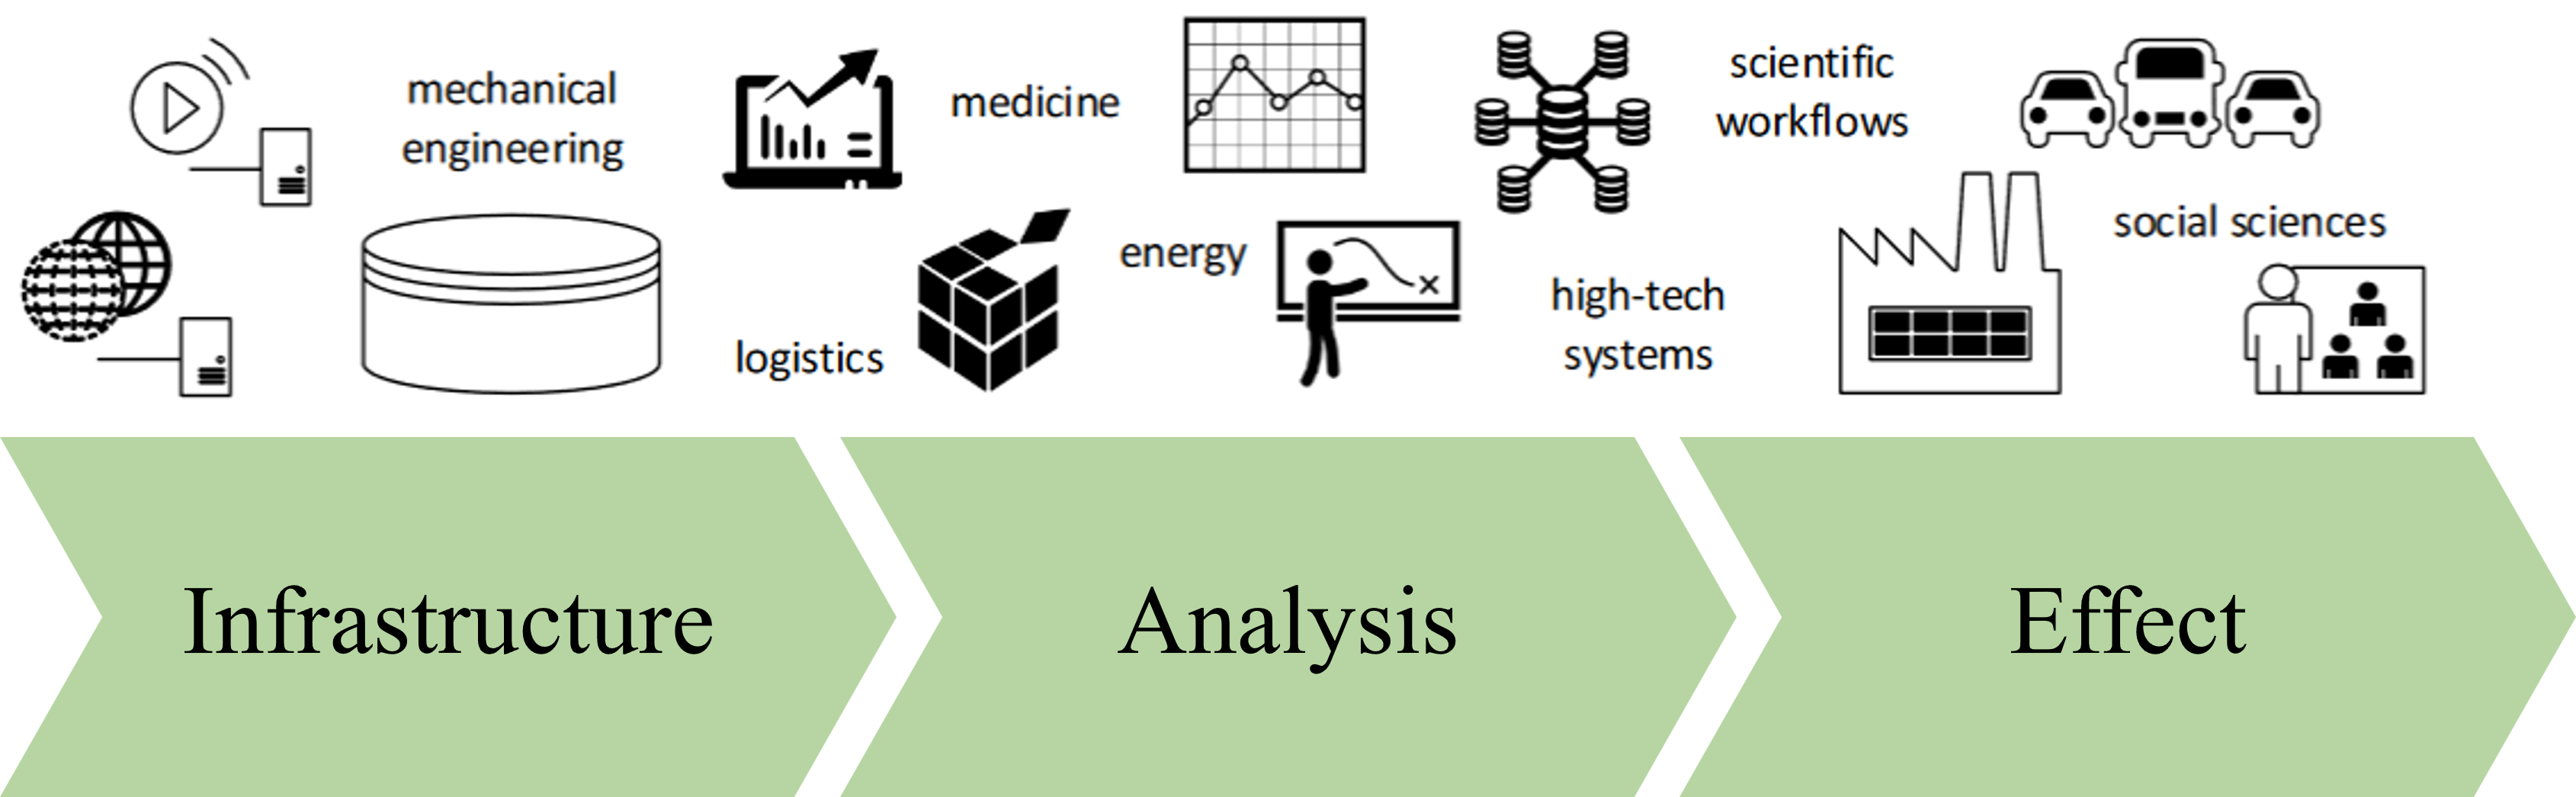
\includegraphics[width=0.75\textwidth]{assets/basics/pipeline.png}
  \caption{Pipeline of data science}
  \label{fig:1_pipeline}
\end{figure}

Let's look at the individual components. The first step to pay attention to when wanting to handle data is the \sidenote{Infrastructure}\textbf{infrastructure} with the keywords \textbf{"volume and velocity"}. The main challenge is making things scalable and instant (responsiveness). Important terms are for example:
\begin{itemize}
  \item Instrumentation
  \item Big data infrastructures, distributed systems
  \item Data engineering (databases and data management)
  \item Programming
  \item Security
\end{itemize}

Next, we have the step of the actual \sidenote{Analysis}\textbf{analysis} concerned with \textbf{extracting knowledge} from data. The core challenge can be put as providing answers to known and unknown unknowns. Important terms are for example:
\begin{itemize}
  \item Statistics, algorithms
  \item Data and process mining
  \item Machine learning, artificial intelligence
  \item Operations research
  \item Visualization
\end{itemize}

Finally, we also need to be concerned with the \sidenote{Effects}\textbf{effect} of our results on people, organizations, and society. The main challenge of this pipeline step is to do \textbf{responsibly} perform data handling. Important terms are for example:
\begin{itemize}
  \item Ethics and privacy, and IT law
  \item Human-technology interaction
  \item Operations management
  \item Business models, entrepreneurship
\end{itemize}

This course will look into all the steps of the pipeline, but the main focus lies on the data analysis.